\section{Process development and flowsheeting}
\label{sec:flowsheeting}

\subsection{Process overview}

Nitroma's process for the production of substituted aromatic amines via nitration is composed of four section, as shown in \cref{fig:BFD}: toluene nitration (red); \ortho-nitrotoluene reduction (green); \para-nitrotoluene partial oxidation and 4-nitrobenzaldehyde reduction (purple); \para-nitrotoluene complete oxidation and 4-nitrobenzoic acid reduction (blue). 


Following the selection of separation techniques and reactor types for each step shown in \cref{fig:BFD}, the process was simulated with ASPEN Plus to obtain approximates for sizing, heat duties and residence times required to meet the production targets. Reaction kinetics were modelled as Arrhenius rate laws with constants and activation energies derived from published work. The thermodynamic property method NRTL was selected because of the presence of polar mixtures. For a plant operating at steady-state 275 days per year, ASPEN simulations found that \SI{652}{\tonne\per\year} of \SI{99}{\percent} pure \ortho-toluidine, \SI{538}{\tonne\per\year} of \SI{99.3}{\percent} pure 4-aminobenzaldehyde and \SI{100}{\tonne\per\year} of pure 4-minobenzoic acid could theoretically be produced by Nitroma's process.


This section will detail the decision making steps taken to determine the optimum reactor types and separation strategies for the development of an inherently safe and continuous process. Particular importance was given to process intensification principles during technology selection, which gave rise to process innovations.

\begin{figure}[htb]
    \centering
    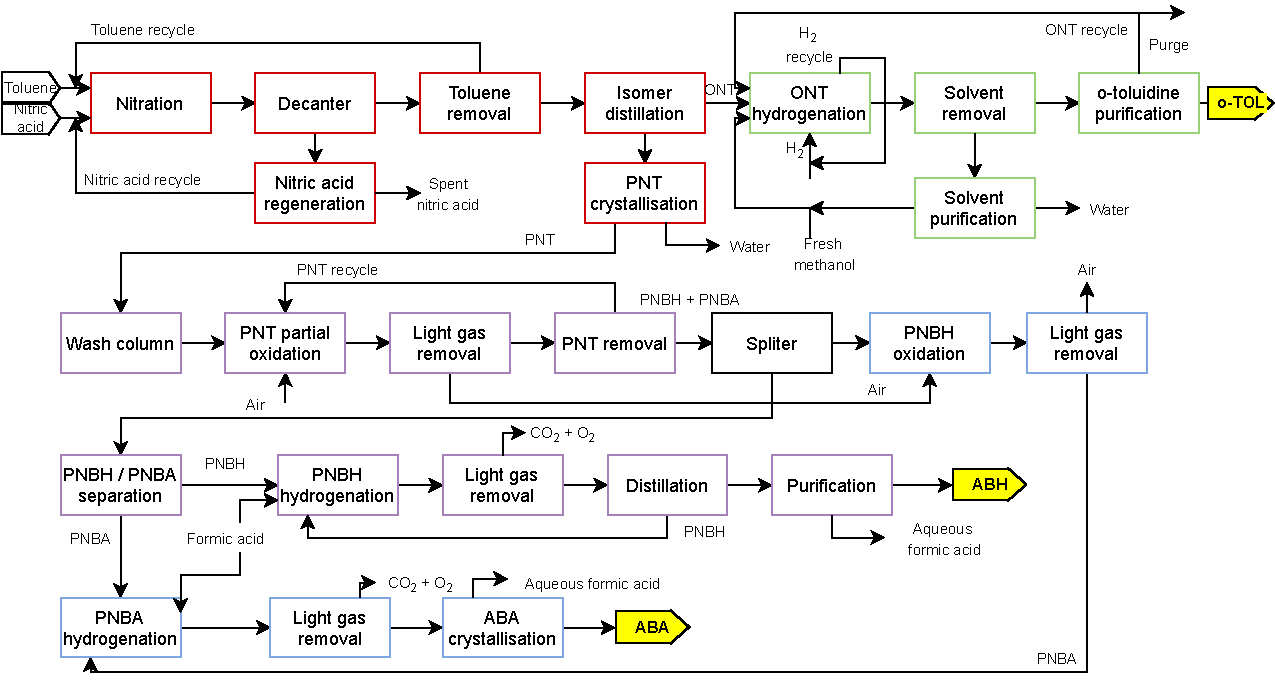
\includegraphics[width=\linewidth]{chapters/1-synthesis/1-Figures/BFD_nitroma-07_03.pdf}
    \caption{Block Flow Diagram of Nitroma's process}
    \label{fig:BFD}
\end{figure}


\subsubsection{Operating mode} % batch vs continuous
\label{sec:continuous}
The first level of decision according to \textcite{douglas_conceptual_1988} is whether to operate a batch or continuous process. On the one hand, a continuous process is designed to operate 24/7 until the plant is shut down for planed maintenance. On the other hand, batch processes are made of several units designed to be started and stopped frequently. Most processes contain a mix of batch and continuous units and one usually refers to a continuous process when only one or two units in a large production plants are operated batch-wise \cite{douglas_conceptual_1988}. 

At industrial scale, nitration is mostly carried out in batch or semi-batch reactors to control the temperature rise caused by the exothermic nature of the reaction \cite{booth_nitro_2000,dugal_nitrobenzene_2005}. However the heat and mass transfer rates are limited in batch reactors, leading to low volumetric productivity, especially for heterogeneous catalysis reactions \cite{randall_process_2020}. Scale-up of the batch process is made very difficult due to inadequate heat transfer area for exothermic reactions; batch to batch variation of conversion, selectivity and yield; prolonged reaction times; and nitrating agent in excess occupying significant reactor volume \cite{kulkarni_continuous_2014}. The large reactor volumes required decrease the safety of the process. Moreover most batch processes are operated sub-optimally to match the equipment capabilities in terms of heat transfer, mass transfer and mixing \cite{randall_process_2020}. Despite the undesirable increased cost, complexity and plant footprint, batch nitration remains the industry standard due to the small scale and occasional production of speciality chemicals. 

Recent studies have demonstrated that some of those challenges can be overcome with continuous flow processing, which would drastically reduce the chemical plant footprint. \textcite{kuba_batch_2007} reported that higher yields could be obtained with continuous nitration of toluene over zeolite beta, thus making this mode of operation very attractive for large-scale production. Selectivity towards the more economically favoured \para-isomer was also found to be increased due to lower contact times suppressing uncatalysed nitration \cite{kuba_batch_2007}. A publication by \textcite{di_miceli_raimondi_safety_2015} highlights the safety improvements offered by continuous flow nitration. In case of failure, the temperature rise is three times lower than for semi-batch and can be better controlled in intensified device for continuous processing. The heat of reaction can be satisfactorily dissipated through the reaction walls, thus avoiding runaway reactions \cite{di_miceli_raimondi_safety_2015}. 

From a process intensification point of view, continuous processes have many potential benefits. As the  reactor is only used for the designed reaction step, downtime for charging and discharging raw materials/products, heating/cooling, phase separation, solvent distillation and equipment cleaning between batches are eliminated \cite{randall_process_2020}. Intensified technologies, such as microreactors and spinning disk reactors, can be adopted when switching from batch to continuous. Moreover, the reduced reactor size has multiple favourable implications on the nitration, hydrogenation and oxidation reactions performed by Nitroma:
\begin{itemize}
    \item The increased surface to volume ratio results in an increased specific heat transfer rate, thus improving the safety thanks to faster heat removal.
    \item The increased mixing intensity leads to higher energy dissipation rates, thus improving safety and productivity.
    \item Product selectivity and quality is increased thanks to more homogeneous mixing and reduced mixing time, which is an advantage for downstream processing and especially crystallisation.
    \item The lower liquid holdup results in less residual heat and thus improved safety.
    \item ``Novel process windows" can appear, enabling the use of intensified process conditions, including higher temperature, pressure and concentrations, as well as the implementation of alternative synthesis routes considered too dangerous from a thermal safety point of view to be carried out in batch reactor.
\end{itemize}
Other economic advantages of continuous processing include: the suppression of intermediate storage and associated equipment; easier heat integration; lower manpower requirements (more automation thanks to steady-state operation); and reduced separation costs thanks to better selectivity.

A list of heuristics has been developed to justify the transfer from batch to continuous processing \cite{randall_process_2020}: highly exothermic reaction; selectivity highly dependant on temperature; presence of hazardous reagent, intermediate or product; and large volume product.
Nitroma's process consists of highly exothermic reactions carried out with hazardous reagents and products present in large volume, thus justifying the consideration of continuous processing. Thanks to the safety, performance and economic benefits offered by a continuous over batch process, it was decided to design an inherently safer continuous process for nitration and subsequent reduction of substituted aromatics.

\subsubsection{Plant modularity} 

Plant modularity refers to the degree of flexibility a process can accommodate. Nitroma will implement this process intensification concept in different aspects of its design. The plant is indeed multipurpose and can produce three valuable amino derivatives of toluene. The productivity of the process can be modified to align with product demand from the different industries where they find application. Nitroma's process is designed to operate in either 4-aminobenzaldehyde or 4-aminobenzoic acid campaigns. The more valuable 4-aminobenzaldehyde is produced through the partial oxidation of PNT and this oxidation can be continued to the benzoic acid counterpart by increasing the residence time. Following the first oxidation, the reactor outlet can either be directed to the PNBH hydrogenation reactor to produce 4-ABH, or to the second oxidation reactor where complete oxidation to PNBA occurs. In order to meet the maximum production target negotiated by Nitroma's, the plant must operate 240 days in the 4-aminobenzaldehyde scenario and 35 days in the 4-aminobenzoic acid scenario. The number of operating days can be adjusted to the current demand for either product, thus offering significant plant versatility. The product purity could also be altered to meet customer requirements.

Another aspect is modular construction, whereby main process equipment is standardised using pre-assembled units transported on site for connection. In order to balance innovation and modularity, Nitroma will design certain reactors and separation units based on standardised commercially available modules while creating novel designs for the nitration reactor and crystallizers. The main advantages offered by modules are the reduction in capital expenditure, faster time to market, simplified maintenance and increased safety since modules are built under controlled conditions and tested prior to shipping \cite{baldea_modular_2017}.

\subsection{Process intensification principles}

Process intensification (PI) refers to any chemical engineering development leading to substantially smaller, cleaner, safer and more energy efficient technology \cite{reay_chapter_2008}. Established in the 1970s with the objective of reducing capital cost by dramatically reducing the plant volume by 100 to 1000-fold, the interest for PI has been constantly growing in the last few years due to the necessity for the chemical industry to design more sustainable processes. Nitroma aimed to develop a process following PI principles wherever applicable to benefit from the numerous advantages which include cheaper and safer processes, smaller equipment and plant, less energy and raw materials consumption, shorter time to market, less wasteful by-products, as well as better company image due to reduced environmental impact \cite{reay_chapter_2008}. PI will also enable Nitroma to leverage recent tax subsidisation policies set by the Chinese Ministry of Commerce related to safe process design \cite{nanjing_economic_and_technological_development_zone_administration_committee_public_2019}.  

The first consideration of process intensification is the conversion of a batch process to a continuous one \cite{randall_process_2020}. As discussed previously in \cref{sec:continuous}, Nitroma's process will be operated continuously in order to benefit from improved safety, economics and product quality. To make this decision, the feasibility of a continuous process was assessed with a method developed by \textcite{teoh_practical_2016}. For each step of the process, equipment were  identified for continuous processing and evaluated in terms of their level of technical difficulties and qualitative benefits. Solutions were ranked from low to high and placed on a decision matrix to inform whether continuous processing would be favourable. This analysis found that all units contained in Nitroma's process can be operated continuously.

The general guiding principle in PI is to maximise the effectiveness of intra- and inter-molecular events and to give the same processing experience to each molecule \cite{randall_process_2020}. PI can be applied to both the hardware and the software of a chemical process, to be said the equipment and the production methods employed \cite{stankiewicz_re-engineering_2003}. The technology can either be for reactive (spinning disk reactor and microreactor) or non-reactive operations (static mixer, COBR crystallizer). Nitroma will aim at following the developed criteria to make informed choices on the different industrialisable technologies, whether they are conventional or PI equipment. The main criteria are: increased heat transfer and decreased holdup of reaction mixture for improved safety; limited uncertainties (maintenance, availability, cost...) and proven reliability and robustness of technology and scale-up feasibility; initial high investment costs must be outweighed by saving in labour costs, energy, inventory and raw materials; improved product quality and selectivity; and increased productivity due to enhances heat and mass transfer \cite{randall_process_2020}. In addition to improving safety, chosen equipment should also contribute in the reduction of safety-related costs, thus enabling Nitroma to offer products below market price whilst maintaining a sufficient profit.

Examples of PI methods include: multifunctional reactors (such as reactive separations and heat-integrated reactors), hybrid separation techniques (membrane adsorption), alternative energy sources (centrifugal field, microwaves, ultrasounds), the use of novel solvents (supercritical fluids and ionic liquids) and greener process synthesis. Regarding the latter, Nitroma has decided to follow as closely as possible the 12 principles of Green Chemistry in the choice of reaction routes \cite{anastas_green_2010}. By selecting solid acid catalysts and in particular safer zeolite for nitration, Nitroma's process is inherently safer, produces less toxic and harmful waste than conventional mixed-acid processes and is more energy efficient. Decision making driven by green chemistry principles is also reflected in the selection of a solvent for ONT reduction, where methanol was preferred due to its more benign and environmentally friendly nature than other alternatives.

Despite the potential improvement offered by PI, its widespread application in industry has been limited due to insufficient know-how and the high technical and financial risks associated with developing a new process \cite{randall_process_2020}. Nitroma will balance the risks and benefits of PI technology when selecting process techniques and equipment for its continuous process.

\nomenclature[A]{PI}{Process intensification}

\subsection{Reactor choices}
\label{sec:reactorchoices}

The choice of reactor type was driven by Process Intensification principles, especially the feasibility of continuous processes, safety aspects and product quality. 

\subsubsection{Nitration reaction} \label{sec:synthesis-R1}

Toluene nitration is a three-phase highly exothermic reaction where mass transfer between the aqueous, acid and solid phases must be maximised while ensuring efficient heat removal to prevent thermal runaway. This section will briefly present the different types of conventional and intensified reactors considered. Further explanations can be found \cref{sec:reaction} where the nitration reactor was designed in great detail.

A conventional continuous reactor for three-phase systems is a stirred slurry reactor, which has an automatic agitator that controls the inflow and outflow of the product. This provides a high degree of automation \cite{liu_nitration_2019}, which is particularly useful when the reaction temperature has to be carefully controlled, as it is the case with toluene nitration. However, in the presence of solid H-Mordenite catalyst, the mechanical agitation will erode the catalyst in the liquid suspension \cite{argyle_heterogeneous_2015}. The catalytic activity would decrease over time resulting in more frequent catalyst regeneration to achieve the same conversion as fresh catalyst. Further, the reactor effluent must be filtered to retain the catalyst in the reactor. 
An alternative to slurry reactors is conventional packed-bed reactor. This reactor is easy to operate because the packed structure of the catalyst removes the need for catalyst filtration in the outlet stream. The compact packing also allows for high zeolite catalyst loading, thus enhancing the rate of reaction \cite{kashid_microstructured_2009}. A simple modelling of a packed-bed reactor usually assumes perfect mixing, however, in reality flow maldistribution and hot spot formation occurs \cite{nguyen_flow_1994}. This is dangerous for the nitration process as any hot spots will promote the thermal runaway process that increases the risk of explosion. 

In line with Nitroma's goal of developing an inherently safer and intensified process, microreactors were considered. Their very high heat transfer rate resulting from the high surface area to volume ratio enable the efficient control of highly exothermic reactions such as nitration \cite{halder_nitration_2007}. Additionally, the reaction can be controlled by intrinsic kinetics only since the mass transfer rate in the microreactor can be high enough to overcome mass transfer limitations \cite{halder_nitration_2007}. Microchannel packed bed reactors were initially considered for heterogeneous reaction but the very high potential pressure drop (\SI{>40}{\bar}) makes their implementation impossible for Nitroma's large scale production \cite{rebrov_microreactors_2016}. Alternative coated wall microreactors and catalytic static mixers were also investigated. However those technologies are in their infancy and have yet to be modelled and scaled-up for industrial production \cite{lopes_regime_2013}. Moreover, experiments have found that the distribution of nitrotoluene isomers with solid acid catalysts in a microreactor was similar to that of mixed-acid nitration, thus losing the benefit of H-Mordenite favouring the more valuable PNT over ONT \cite{halder_nitration_2007}.


A hybrid alternative which offers the benefits of a packed-bed reactor, while preventing the possibility of hot spot formation through enhanced heat transfer ability resides in intensified heat exchangers (HEX) reactors \cite{di_miceli_raimondi_safety_2015}. Their design is largely based on conventional heat exchanger geometries including plate-type and shell-and-tube (S\&T) heat exchangers \cite{anxionnaz_heat_2008}. Plate HEX demonstrate higher heat transfer coefficient than S\&T resulting in less surface area required for a given heat duty, thus decreasing the overall volume and costs. However catalyst coating of the heat transfer surface in plate HEX is problematic since the catalyst will deteriorate during operation and will need regeneration which is challenging for coated wall reactors \cite{anxionnaz_heat_2008}. Conversely, shell-and-tube heat exchangers with catalyst inserts in tubes can overcome this challenge. The interest in this technology has been growing due to the improved heat transfer without a pressure drop as significant as in microchannel reactors \cite{griffin_heat_2001}. Mixing can also be improved depending on the type of specific inserts used in the tubes. Those multifunctional apparatuses have been designed for catalytic exothermic reaction as they can fulfil the requirements for safe, selective and energy efficiency processes \cite{anxionnaz_heat_2008}. Based on those considerations, Nitroma will design and implement a shell-and-tube heat exchanger reactor for the nitration of toluene over H-Mordenite catalyst.

\nomenclature[A]{MNT}{3-nitrotoluene, \meta-nitrotoluene}

\subsubsection{\ortho-toluidine production} \label{sec:otol}

The hydrogenation of ONT is a three-phase system comprising liquid ONT mixed with methanol solvent, gaseous \ch{H2} and solid Pd/C catalyst. Three-phase catalytic reactors can be classified in two main types: suspended catalyst in the liquid (slurry reactor) or fixed bed catalyst (trickle or packed bed reactors) \cite{wood_methodological_nodate}. 

The slurry reactor provides a steady agitation of the reaction, favourably increasing the selectivity \cite{p_a_ramachandran_recent_1987}. However violent agitation also results in solid Pd/C catalyst attrition, which is very undesirable due to the high cost of precious metal Pd. Catalyst regeneration would indeed be very expensive thus lowering the economic potential (EP) of this plant. Moreover, based on the kinetics of the oxidation reaction derived from  \textcite{rajadhyaksha_solvent_1986}, the rate constant is strongly dependent on the mass of Pd catalyst, further emphasising the importance of low catalyst attrition. Similar drawbacks have been observed for other types of suspended catalyst reactors. Despite enhanced heat and mass transfer and optimal fluid-solid contact increasing reaction efficiency, fluidised bed reactors was deemed an unsatisfactory option due to significant catalyst erosion resulting in performance losses. The presence of liquid ONT would cause heavy components to deposit on the catalyst, reducing the effectiveness of the Pd catalyst and leading to increased agglomeration, even more so than in slurry reactors \cite{farrell_kinetics_1979}. The latter can however be found more suitable for gas-phased hydrogenation with the usage of \ch{H2} gas at lower pressures, which is not applicable in the current liquid-phase hydrogenation operating at high pressures (\SI{5}{\atm}) \cite{ranade_chapter_2011}.

Conversely, trickle bed reactors are known for their ease of operation at high pressure and the slow catalyst deactivation, which is imperative for an expensive catalyst usage of Pd/C \cite{vemala_hydrodynamic_nodate}. Furthermore, the liquid plug flow behaviour in trickle bed reactor allows for high conversion, thus increasing the final production rate of o-TOL. Trickle bed reactors can be operated in a co-current or counter-current fashion. Counter-current operation can increase overall performance of the reactor by improving catalyst wetting \cite{kundu_novel_2003}. However, the risk of flooding, where counter-current phase is reversed, is not negligible due to the strong interfacial friction between upward moving gas and downward moving liquid \cite{breijer_prevention_2008}. Co-current flow significantly reduces the risk of flooding, thus allowing for higher flowrates of products \cite{vemala_hydrodynamic_nodate}. As the risk of flooding offsets the benefits provided by counter-current flow, it was thus decided to perform ONT hydrogenation in a co-current trickle bed reactor (R201) operating at \SI{333}{\K} and \SI{5}{\atm} with both gas and liquid in downflow mode. 

\nomenclature[A]{EP}{Economic potential}

\subsubsection{Oxidation and hydrogenation of PNT derivatives} \label{sec:synthesis-R3-R4}

The reactor for the gas-phase oxidation of PNT with air over solid cobalt phthalocyanine catalyst must be carefully selected in order to control the partial oxidation to 4-NBH, while accommodating the complete oxidation to 4-NBA. High selectivity should be obtained at high conversions while minimising reactor size and eliminating thermal runaways caused by high heat generation \cite{schmidt_catalytic_1994}. Other favourable attributes for oxidation reactors include high mass and heat transfer rates and narrow residence time distributions. The two main types of gas-solid reactors can be distinguished based on the solid catalyst system: suspended particles as in fluidized bed reactors, and structured packing of pellets. Since cobalt is a relatively expensive metal \cite{saib_fundamental_2014}, catalyst attrition must be minimised to ensure economic viability of the process. The large flowrates required in fluidised bed reactors dramatically increase catalyst erosion, thus making it an unattractive option. This problem is less prevalent in packed-bed reactors, which are more preferable. Despite large concentration and temperature gradients in packed bed partial oxidation reactors, the residence time distribution can be controlled to achieve the optimum residence time for partial oxidation of PNT to 4-NBH \cite{schmidt_catalytic_1994}.

Liquid-phase hydrogenation of 4-NBH and 4-NBA using formic acid as the transfer hydrogen donor and Pt/C as catalyst at room conditions can be performed in reactors similar to those described for ONT reduction (see \cref{sec:otol}). In addition to the aforementioned benefits, continuous flow hydrogenation in a packed-bed reactor allows for good recovery of catalyst, as investigations have shown that recycled catalyst has a similar efficiency as fresh catalyst \cite{rahman_fast_2020}. This is of paramount importance for this reaction as the constant regeneration of expensive Pt catalyst could greatly decrease the economic potential \cite{rahman_fast_2020}. 


\subsection{Separation strategies}

To select the optimal separation techniques for its continuous process, Nitroma ranked the different options using the Jaksland procedure. This method was chosen as a quantitative method of ranking separation techniques because it is well established and does not require much computation once physical properties of the chemicals are known \cite{jaksland_separation_1995}. 

\subsubsection{Nitrotoluene isomers}

The first separation step of the process is the recovery of spend  aqueous nitric acid from the organic phase in a decanter. Following water evaporation in a distillation column (S102), nitric acid is recycled back into the nitration reactor at a \SI{94}{mol\percent} purity. Nitroma decided to employ the most common acid regenartion process employed by industry \cite{dugal_nitrobenzene_2005}. Meanwhile, the organic phase is sent to a distillation column (S103) recovering \SI{99.8}{mol\percent} toluene from the less volatile nitrotoluenes, which is fed back to the nitration reactor, following standard industrial procedures \cite{bowers_toluidines_2000}.

The nitrotoluene isomer separation is a crucial step, as it determines the production rate of downstream products. Thus the separation techniques above were carefully selected using both the Jaksland quantitative analysis \cite{jaksland_separation_1995} and sound engineering judgement. Separation across different phases such as vapour-vapour, vapour-liquid, liquid-liquid and liquid-solid were considered, as shown in \cref{tab:separation techniques} in \cref{app:jaksland}. Based on thermodynamic insights, a binary ratio matrix was computed using physical data from the literature. The property pair ratios for the compounds involved in this section of Nitroma's process are shown in \cref{tab:jaksland}. Properties investigated include critical and triple point temperatures, boiling and melting points, vapour pressure, critical pressure, water solubility, molecular weight and heat of vaporisation \cite{jaksland_separation_1995}. The relevant property pair ratios were then compared against the feasible and good bounds for each of the shortlisted techniques, which are tabulated in \cref{tab:separation-pair-ratio}. Finally, the $\mu$ value for each feasible technique is calculated and tabulated in \cref{tab:separation-mu}, and the technique with the highest value is considered to be the most optimal. 

\begin{table}[h]
\centering
\caption{$\mu$ values for each shortlisted technique.}
\label{tab:separation-mu}\footnotesize
\begin{tabular}{@{}llllll@{}}
\toprule
Pair              & Distillation                 & Distillation                    & Flash      & Flash      & Crystallisation (melt) \\ \midrule
Criteria             & Boiling point                &     Vapour pressure           & Boiling point       & Vapour pressure          & Melting point \\ \midrule
ONT / PNT & 2.23                         & \cellcolor[HTML]{C6E0B4}37.88   & Infeasible & 1.62       & 0.11                   \\
ONT / MNT & 0.89                         & \cellcolor[HTML]{C6E0B4}45.42   & Infeasible & 2.30       & Infeasible             \\
PNT/ MNT & \cellcolor[HTML]{C6E0B4}0.32 & 0.31                            & Infeasible & Infeasible & Infeasible             \\
ONT / tol     & 27.97                        & \cellcolor[HTML]{C6E0B4}6665.48 & 0.35       & 598.10     & 4.43                   \\
PNT / tol     & 32.14                        & \cellcolor[HTML]{C6E0B4}366.12  & 0.60       & 31.16      & 8.90                   \\
MNT / tol     & 30.41                        & \cellcolor[HTML]{C6E0B4}307.95  & 0.49       & 25.93      & 6.00                   \\ \bottomrule
\end{tabular}
\end{table}

Decanting of the three nitrotoluene isomers was ruled out as an option because the organic molecules were very likely miscible with each other \cite{merck_solvent_2021}. Although certain adsorbents have proved to be able to preferentially adsorb ONT and PNT, further purification steps would be required to desorb and separate the nitrotoluenes from the desorbent \cite{zhao_new_2016}. The available literature recommends using distillation to remove the desorbent, which seems to make adsorption a redundant step compared to direct distillation of the nitrotoluene isomers \cite{zinnen_ep0181106a2_1984}. Absorption was also not considered as the solubility of the nitrotoluene isomers are similar across different types of solvents since the functional groups and molecular weights of the isomers are identical. Sedimentation was not considered as the maximum purity achievable is around \SI{70}{\percent} \cite{seider_product_2009}. Instead, crystallisation is a relatively new separation technique which was considered. 

From the shortlisted techniques presented in \cref{tab:separation-mu}, distillation based on vapour pressure differences appears as optimum for most pairs of components. Although the Jaksland analysis recommends that distillation be used to separate m and \para-nitrotoluene, the boiling point difference between the two compounds at \SI{1}{\atm} was only \SI{7}{\K}. In contrast, their melting points differed by \SI{36}{\K}. The larger difference in melting points suggested that melt crystallisation would be an easier separation, and would potentially provide a cleaner split between the two isomers. This seems to be the reason why crystallisation is a widely adopted strategy to separate MNT and PNT after distilling off ONT \cite{weiland_purification_1931,european_chemical_agency_background_2010}. 

Based on these considerations, Nitroma decided to implement the following separation sequence for nitrotoluene isomers: the nitrotoluenes are sent to a distillation column to separate \SI{99.99}{mol\percent} of the more volatile ONT from MNT and PNT which are then separated by crystallisation, thus exploiting the large difference between their melting points.

Two main types of crystallisation techniques were explored: melt crystallisers and solution crystallisers. In both cases, crystal growth rates are relatively fast resulting in high product purity which is economically favourable. From an environmental point of view, solution crystallisation is less favourable as it often involves the addition of a solvent which is usually treated as impurity, whereas melt crystallisation does not require any additional substance. However Nitroma aims at developing a continuous process and as such a suspension crystalliser which can be operated continuously was preferred. Further considerations for the choice of crystallisation equipment can be found in \cref{sec:separation}. A novel crystalliser known as mixed-suspension mixed-product removal (MSMPR) was finally chosen since it is a compromise between the two techniques: no additional solvent is required thus improving the environmental impact, and continuous operation is feasible. A slurry of PNT crystals and MNT liquid is continuously produced, followed by liquid separation in a hydraulic wash column to attain purified molten \para-nitrotoluene. This technology was found to provide significant process intensification advantages: it is more compact than solid layer crystallisers, has as smaller energy consumption and can be operated continuously.

\subsubsection{After 4-nitrotoluene oxidation}

Following crystallisation and melting in a wash column, PNT was partially oxidized to PNBH with the option of complete oxidation to PNBA. In both scenarios, the effluent from the oxidation reactor is sent to a flash drum that removes air and water vapour from the organic stream. In the case of partial oxidation, the organic stream is then fed into a distillation column, where \SI{99.9}{mol\percent} of the unreacted PNT is separated from the less volatile nitroaromatics and recycled to the reactor. 
In the 4-ABH scenario, PNBH is separated from inevitable complete oxidation product PNBA in a distillation column. The PNBH and PNBA are then fed to their respective hydrogenation reactors. Distillation was found to be the most favourable separation technique based on the Jaksland analysis.


\subsubsection{Products recovery}

The effluent from the PNBH hydrogenation reactor is sent to a flash drum (S501) to remove air and water vapour. Then, two distillation columns are employed to remove unreacted PNBH and remaining water to yield  \SI{99.9}{mol\percent} pure 4-ABH. On a molar basis, \SI{97}{\percent} of the 4-ABH produced in the reactor can be recovered at the end of the separation. The unreacted  PNBH was recycled back to the hydrogenation reactor to improve the production yield.

In the ABA scenario, the liquid effluent from reactor the hydrogenation reactor is sent to a continuous falling-film melt crystalliser to recover \SI{96}{mol\percent} of 4-ABA in the form of pure solid crystals. In this instance, distillation was found to require a very high heat duty due to the large amount of water present, thus making crystallisation more attractive to purify 4-ABA. 

Following reduction of ONT, o-TOL is purified to meet the purity requirement of \SI{98}{mol\percent}.
The hydrogen gas leaves the reactor via an outlet port, and the effluent enters a distillation column to separate methanol and water from the less volatile organic compounds.
Finally, a second distillation column removes \SI{94.8}{mol\percent} of unreacted ONT which is recycled, yielding a \SI{99.4}{mol\percent} pure o-TOL product. Finally, the methanol solvent is stripped from water to be recycled.

All the columns involved in the process were designed as packed column due to improved heat and mass transfer resulting in equipment of smaller sizes for the same performance as plate columns. Nitroma viewed this advantage positively in its effort in designing an intensified process for the production of substituted aromatic amines.

\subsection{Heat integration}

\begin{wrapfigure}{r}{0pt}
    \vspace{-\intextsep}
    \centering
    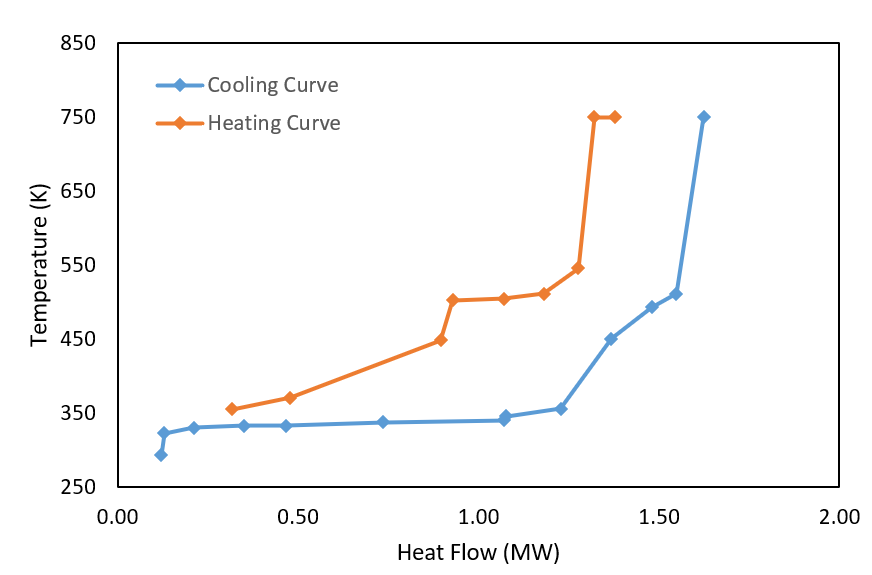
\includegraphics[width=0.48\textwidth]{chapters/1-synthesis/1-Figures/composite-curves.PNG}
    \caption{Composite curves of heat transfer equipment}
    \label{fig:heat}
\end{wrapfigure}

Prior to energy saving considerations, the plant requires an approximate annual net heating duty of \SI{2.65}{\MW}. Hence, pinch analysis has been conducted in the attempt to reduce utility costs and carbon emission, as seen in \cref{fig:heat}. However, it has been decided to not integrate process streams due to following reasons. First of all, temperature is critical to all process units in both performance and safety aspects. Temperature disturbance in one stream could cause a major disruption on a different section if the streams are integrated. Also, given the small flowrate across the plant, economic cost of constructing a comprehensive heat exchange network outweighs the utility cost due to the expensive costs of installation and maintenance of heat exchangers.

 Instead, Nitroma has considered reducing energy input by recovering thermal energy from used utility stream. It has been identified that the cooling water exiting several heat removal units has significant heat residue to supply a the reboiler of the methanol recovery column and reduce \SI{0.3}{\MW} of energy input. Heating supply during start-up procedure has been taken into account as well. The aforementioned reboiler is also equipped with a high pressure steam supply that will be activated when the cooling water has insufficient enthalpy. Other coolers and heaters installed are equipped with independent energy transfer system and hence backup equipment is considered unnecessary.

\section{Points of innovation}

\subsection{Continuous multipurpose process}
Nitration of substituted amines is typically an industrial batch process due to the high risk of thermal runaway if the highly exothermic reaction gets out of control \cite{dugal_nitrobenzene_2005}. Scale-up of batch processes is difficult due to safety and performance problems arising from the large reactor volumes required. To overcome those challenges and meet market demand, Nitroma designed an entirely continuous multipurpose process for the nitration of toluene and subsequent reduction to aromatic amines. Continuous flow nitration provides a clear safety advantage as the heat of reaction can be efficiently removed thus avoiding deadly thermal runaways. Moreover, the continuous process developed by Nitroma results in intensified equipment of smaller size thus reducing the plant's footprint and investment costs. Finally, Nitroma's process offers production flexibility thanks to the controlled oxidation of PNT to its partial and complete oxidation products, respectively PNBH and PNBA. The multipurpose plant is thus capable of adapting the production based on market demand, a novel characteristic which is expected to be more and more prevalent in the chemical industry of the future.

\subsection{Zeolite catalysed nitration}

Nitroma decided to move away from the industry standard of performing nitration with a mixed-acid process involving hazardous sulfuric acid. Instead, a novel reaction catalyst by H-Mordenite zeolite was scaled-up. The environmental impact of the process is dramatically improved due to the absence of \ch{NO_x} emissions and the reduction of wasteful spent acid. Moreover the heterogeneous reaction favours the more economically viable para isomer. Nitroma's scaled-up zeolite catalysed nitration process is innovative and will receive intellectual property protection for this novelty. 

\subsection{Continuous reactor for nitration}

To perform a safe and continuous heterogeneous nitration reaction, a novel reactor was designed by Nitroma. A shell-and-tube reactor was developed to ensure satisfactory heat and mass transfer to safely produce nitrotoluenes. This multifunctional device responds to Nitroma's commitment to apply process intensification principles during the design phase. This unique nitration reactor enables a safe, selective and energy efficiency process.
